%!TEX program = xelatex
% ============================================================================
% JIPS (Journal of Information Processing Systems) submission template
% LaTeX reproduction of JIPS_Format(submission)-2024-1.docx
%
% Style   : jips.sty  (page geometry, fonts, colors, headings, headers/footers,
%                      first-page band/footnote block, bio/reference layout)
% Fonts   : ./fonts/  (self-contained; see jips.sty header)
% Refs    : reference.bib  (BibTeX, IEEEtran.bst, numeric [N] labels)
%
% Compile : xelatex -> bibtex -> xelatex -> xelatex   (recommended, real fonts)
%           pdflatex fallback works the same way with substitute fonts.
% ============================================================================
\documentclass[10pt,twoside]{article}
\usepackage{jips}

\hypersetup{pdftitle={Fast Device Discovery for Remote Device Management in
                      Lighting Control Networks}}

\jipsrunningtitle{Fast Device Discovery for Remote Device Management in Lighting Control Networks}
\jipsrunningauthors{Sang-Il Choi, Sanghun Lee, Seok-Joo Koh, Sang-Kyu Lim, Insu Kim, and Tae-Gyu Kang}

\begin{document}

% ============================ FIRST PAGE ====================================
\jipsfirstpage{%
{\fontsize{5}{6.4}\selectfont
\jipsrefmark\ This is an Open Access article distributed under the terms of
the Creative Commons Attribution Non-Commercial License
(\href{http://creativecommons.org/licenses/by-nc/3.0/}{\color{black}http://creativecommons.org/licenses/by-nc/3.0/})
which permits unrestricted non-commercial use, distribution, and reproduction
in any medium, provided the original work is properly cited.\par}
{\fontsize{6}{7.4}\selectfont
Manuscript received Month 06, 20XX; first revision Month 08, 20XX; accepted
Month 06, 20XX.\par
\textbf{Corresponding Author:} Seok-Joo Koh (sjkoh@knu.ac.kr)\par
\textsuperscript{1} School of Computer Science and Engineering, Kyungpook
National University, Daegu, Korea (jips@kips.or.kr, jips1@kips.or.kr,
jips2@kips.or.kr)\par
\textsuperscript{2} Dept. of Computer Science, Zhejiang Wanli University,
Ningbo, China (jips3@kips.or.kr)\par
\textsuperscript{3} LED Communication Research Team, Electronics and
Telecommunications Research Institute, Daejeon, Korea (jips3@kips.or.kr)\par}}

% ------------------------- title and authors -------------------------------
\jipstitleblock{%
Fast Device Discovery for Remote Device Management\\
in Lighting Control Networks}{%
Sang-Il Choi\textsuperscript{1}, Sanghun Lee\textsuperscript{2}, Seok-Joo Koh\textsuperscript{3},\\
Insu Kim\textsuperscript{1}, and Tae-Gyu Kang\textsuperscript{1}}

% ---------------------------- abstract block -------------------------------
\begin{jipsabstract}
The Remote Device Management (RDM) protocol is used to manage the devices in
the lighting control networks. RDM provides bi-directional communications
between a controller and many lighting devices over the DMX512-A network. In
RDM, using a simple binary search scheme, which is based on the 48-bit unique
ID (UID) of each device, discovers the lighting devices. However, the existing
binary search scheme tends to require a large delay in the device discovery
process. In this paper, we propose a novel partition-based discovery scheme
for fast device discovery in RDM. In the proposed scheme, all devices are
divided into several partitions as per the device UID, and the controller
performs device discovery for each partition by configuring a response timer
that each device will use. From numerical simulations, we can see that there
is an optimal number of partitions to minimize the device discovery time for a
given number of devices in the proposed scheme, and also that the proposed
partition-based scheme can reduce the device discovery time, as compared to
the existing binary search scheme.
\end{jipsabstract}

\jipskeywords{Device Discovery, Partition-Based, RDM}

% ============================== 1. INTRODUCTION =============================
\section{Introduction}

One of the primary issues in the lighting control network is how to
effectively manage a lot of devices within the network. Some protocols for
device management have so far been made in the PLASA Technical Standards
Program (TSP) \cite{ref1}, which includes the Digital Multiplex 512-A
(DMX512-A) \cite{ref2} and Remote Device Management (RDM) \cite{ref3}.

The RDM protocol is performed based on the polling system, in which a
controller initiates communication and the devices will respond to the request
of controller. RDM is used for the discovery and management of devices that
are connected through the DMX512-A link. For device discovery, the controller
uses a simple binary search scheme, based on the 48-bit unique ID (UID).
However, this device discovery scheme tends to require a lengthy discovery
time due to exploring the $2^{48}$ theoretically

This paper is organized as follows: Section 2 discusses the existing device
discovery scheme. In Section 3, we propose the fast device discovery scheme
for RDM. In Section 4, we analyze and compare the existing and proposed
schemes in terms of device discovery times. Section 5 concludes this paper.

% ================= 2. EXISTING DEVICE DISCOVERY SCHEME ======================
\section{Existing Device Discovery Scheme}

In RDM \cite{ref3}, a simple binary search scheme is used for device
discovery, which is based on the 48-bit UID of each device. Fig.~1 shows the
existing device discovery scheme, in which a controller performs a binary
search for devices with the UIDs ranging from 0 to $2^{48}$.

\subsection{Wavelet Filterbank}

Initially, the controller sets the UID \textit{search range} with
(\textit{lower, upper}) and sends a discovery message to all of the devices in
the RDM network. If the controller responds to a single response message, the
corresponding device will be successfully found. Otherwise, if two or more
devices have responded at the same time, the controller cannot process the
multiple response messages due to the characteristics of the DMX512-A link
\cite{ref2}. This is because the DMX512-A link does not use the packet
scheduling functionality and thus, multiple response messages will be simply
corrupted and discarded by the controller. In this case, the controller will
further divide the UID search range into the two parts.

\begin{figure}[H]
\centering
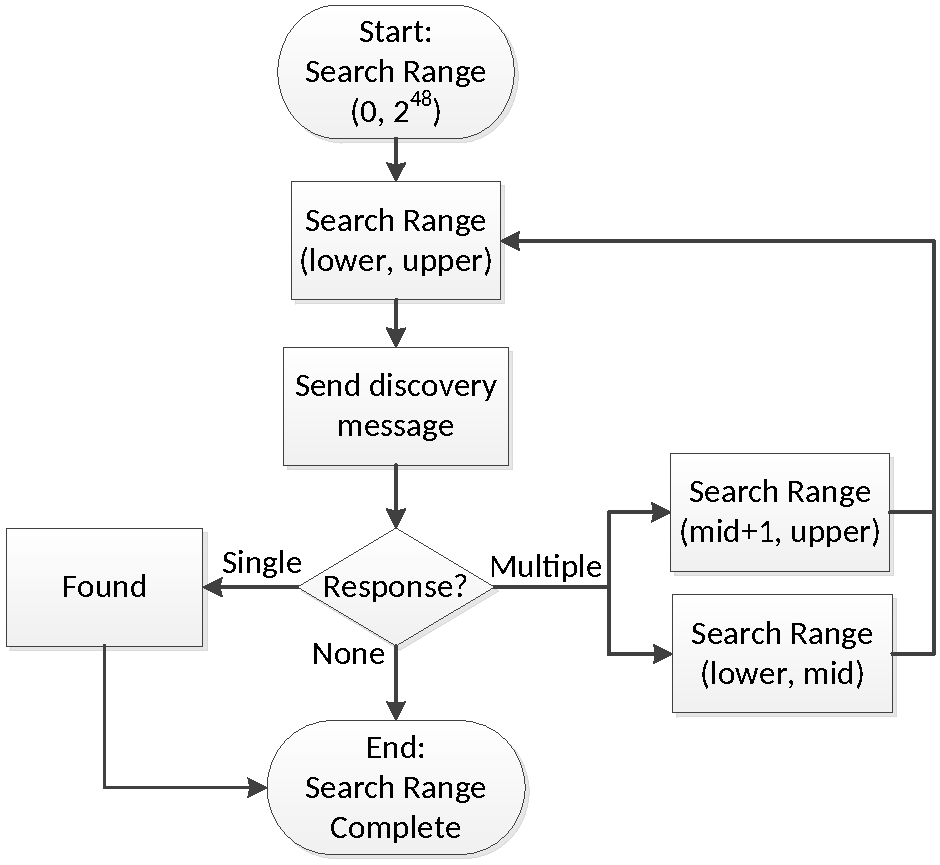
\includegraphics[width=95.2mm,height=71.3mm]{figs/fig1.pdf}
\caption{Existing device discovery in Remote Device Management (RDM).}
\end{figure}

\subsubsection{Wavelet theory}

One of the primary issues in the lighting control network is how to
effectively manage a lot of devices within the network.

% ================= 3. PROPOSED DEVICE DISCOVERY SCHEME ======================
\section{Proposed Device Discovery Scheme}

The existing device discovery scheme gives a lengthy device discovery time
because the 48-bit UID search range ($2^{48}$) tends to induce very deep tree
levels along the binary search tree. Thus, we propose a new device discovery
scheme, called \textit{partition-based} device discovery.

In the proposed scheme, all devices in the network will be grouped into
$N_p$ partitions, as shown in Fig.~2.

\begin{figure}[H]
\centering
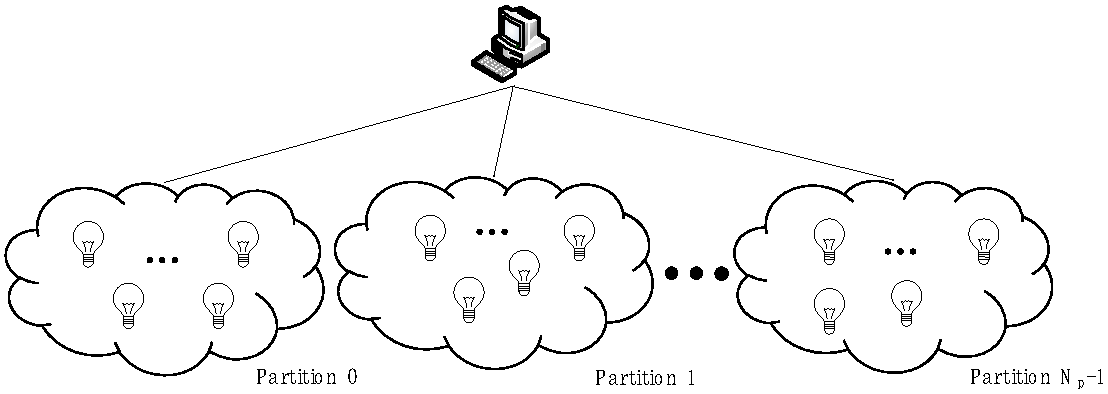
\includegraphics[width=112mm,height=39.2mm]{figs/fig2.pdf}
\caption{Partitions of devices in Remote Device Management (RDM).}
\end{figure}

\noindent
Given the number of partitions ($N_p$), the partition of a device
(0, 1, .., $N_p$-1) is determined by using the \textit{modulo} (\%) operator
and the device UID, as follows:

\begin{center}
\itshape Partition of device UID = UID \% N\textsubscript{p}.
\end{center}

% ========================= 4. PERFORMANCE ANALYSIS ==========================
\section{Performance Analysis}

To evaluate the performance of the proposed scheme, we compared the device
discovery time for the existing binary search scheme and the proposed
partition-based scheme in a variety of network conditions. For numerical
analysis, we used MATLAB (MathWorks, Natick, MA, USA), and we performed five
test instances and obtained the averaged values in simulations.

\begin{equation}
S=201\log_{10}\left(\frac{256}{\varepsilon}\right),\;
\varepsilon=\sqrt{\frac{1}{N^{2}}\left(S_{k}-D_{k}\right)^{2}}
\end{equation}

\begin{equation}
S=201\log_{10}\left(\frac{256}{\varepsilon}\right),\;
\varepsilon=\sqrt{\frac{1}{N^{2}}\left(S_{k}-D_{k}\right)^{2}}
\end{equation}

In our analysis, we first examined an optimal configuration of the parameters
that are used in the proposed scheme, such as the \textit{Delay Increase
Interval} (\textit{DII}) and the number of partitions ($N_p$). After that, we
compared the proposed scheme with the existing scheme in terms of device
discovery time.

Fig.~4 shows the impacts of both $N_p$ and the number of devices on the device
discovery time, in which \textit{DII} is set to 10 time slots. It is noted in
the figure that the device discovery time is plotted in the time unit of
seconds, whereas, the basic operational time unit is 0.0028 seconds in each
simulation. From this figure, we can see that the device discovery time tends
go higher, as the number of devices increases. From the results, it is noted
that there may be an optimal number of $N_p$ for a given number of devices.
For example, for $2^{10}$ devices, $N_p$ = 3 gives the best performance,
whereas, the device discovery time can be minimized at $N_p$ = 6 when there
are $2^{12}$ devices in the network. In our analysis, we first examined an
optimal configuration of the parameters that are used in the proposed scheme,
such as the \textit{Delay Increase Interval} (\textit{DII}) and the number of
partitions ($N_p$). After that, we compared the proposed scheme with the
existing scheme in terms of device discovery time. Fig.~4 shows the impacts of
both $N_p$ and the number of devices on the device discovery time, in which
\textit{DII} is set to 10 time slots. It is noted in the figure that the
device discovery time is plotted in the time unit of seconds, whereas, the
basic operational time unit is 0.0028 seconds in each simulation. From this
figure, we can see that the device discovery time tends go higher, as the
number of devices increases. From the results, it is noted that there may be
an optimal number of $N_p$ for a given number of devices. For example, for
$2^{10}$ devices, $N_p$ = 3 gives the best performance, whereas, the device
discovery time can be minimized at $N_p$ = 6 when there are $2^{12}$ devices
in the network.

\setcounter{figure}{3}% the template numbering jumps from Fig. 2 to Fig. 4
\begin{figure}[H]
\centering
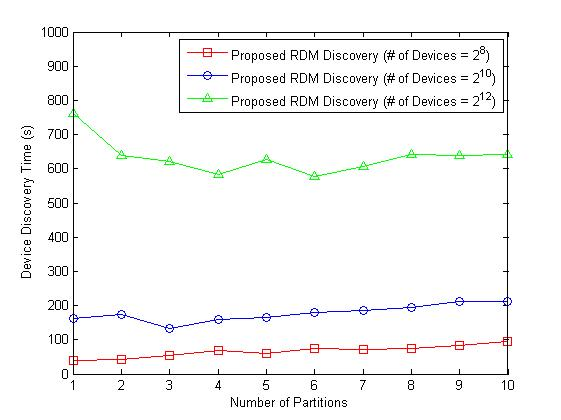
\includegraphics[width=111.1mm,height=75.9mm]{figs/fig4.jpg}
\caption{The impacts of both N\textsubscript{p} and the number of devices on
the discovery time.}
\end{figure}

With this obtained optimal configuration, we compared the overall device
discovery time for the existing binary search scheme and the proposed
partition-based scheme, as shown in Table~1. From this figure, we can see that
the proposed scheme gives a much smaller device discovery time than the
existing scheme does.

\begin{table}[H]
\captionsetup{justification=raggedright,singlelinecheck=false}
\caption{PSNR results [dB] for various test images and $\updelta$ value}
\centering
{\fontsize{8.5}{10.2}\selectfont
\setlength{\tabcolsep}{2pt}
\renewcommand{\arraystretch}{1.15}
\begin{tabular}{@{}
    >{\raggedright\arraybackslash}p{15.5mm}
    >{\centering\arraybackslash}p{5mm}
    >{\centering\arraybackslash}p{14.9mm}
    >{\centering\arraybackslash}p{14.9mm}
    >{\centering\arraybackslash}p{14.9mm}
    >{\centering\arraybackslash}p{14.9mm}
    >{\centering\arraybackslash}p{14.9mm}
    >{\centering\arraybackslash}p{14.9mm}
    >{\centering\arraybackslash}p{14.9mm}@{}}
\toprule
\rowcolor{tabgray}
 & $\updelta$ & Visu-shrink & Sure-shrink & Bayes- shrink & Sendur's method
 & Oracle- shrink & Wiener & Normal shrink \\
\midrule
\multirow[t]{3}{*}{Lena}     & 10 & 28.76 & 33.28 & 33.32 & 33.94 & 33.61 & 33.53 & 33.57 \\
                             & 20 & 26.46 & 30.22 & 30.17 & 30.73 & 30.38 & 30.35 & 28.98 \\
                             & 30 & 25.14 & 28.38 & 28.48 & 28.94 & 28.60 & 28.53 & 25.69 \\
\rowcolor{tabgray}
\multirow[t]{3}{*}{Barbara}  & 10 & 24.81 & 30.21 & 30.86 & 31.13 & 31.50 & 31.37 & 29.81 \\
\rowcolor{tabgray}
                             & 20 & 22.81 & 25.91 & 27.13 & 27.25 & 27.40 & 27.32 & 26.79 \\
\rowcolor{tabgray}
                             & 30 & 22.00 & 24.33 & 25.16 & 25.21 & 25.32 & 25.22 & 24.29 \\
\multirow[t]{3}{*}{Boat}     & 10 & 26.49 & 31.19 & 31.80 & 32.25 & N/A & N/A & N/A \\
                             & 20 & 24.43 & 28.14 & 28.48 & 28.93 & N/A & N/A & N/A \\
                             & 30 & 23.33 & 26.52 & 26.60 & 27.11 & N/A & N/A & N/A \\
\rowcolor{tabgray}
\multirow[t]{3}{*}{Goldhill} & 10 & N/A & 31.87 & 31.90 & N/A & 31.97 & 31.71 & 31.80 \\
\rowcolor{tabgray}
                             & 20 & N/A & 28.43 & 28.65 & N/A & 28.76 & 28.65 & 28.26 \\
\rowcolor{tabgray}
                             & 30 & N/A & 27.02 & 27.11 & N/A & 27.16 & 27.09 & 27.09 \\
\bottomrule
\end{tabular}}
\end{table}

% =============================== 5. CONCLUSION ==============================
\section{Conclusion}

In this paper, we have proposed a new partition-based device discovery scheme
in lighting control networks. In the proposed scheme, all devices are divided
into several partitions. In addition, to avoid collisions occurring due to
multiple responses, each device sends a response message based on a response
timer that is configured by the controller.

From the numerical analysis, we can see that the proposed scheme can provide a
much lower device discovery time than the existing scheme. Moreover, the
performance gaps between the existing and proposed schemes become lager, as
the number of devices increase.

% ============================== BACK MATTER =================================
\section*{Conflict of Interest}

\vspace{9mm}

\section*{Funding}

Please describe the sources of funding that have supported the work.

\vspace{9mm}

\section*{Acknowledgments (optional)}

\vspace{9mm}

% ============================== REFERENCES ==================================
% refs 4-5 are listed in the template without being cited in the body text
\nocite{ref4,ref5}
\jipsbibliography{reference}

% =========================== AUTHOR BIOGRAPHIES =============================
\vspace{6mm}

\jipsbio{figs/photo.png}{Sang-Il Choi}{https://orcid.org/0000-0002-4510-0385}{%
He received B.S. and M.S. degrees in School of Computer Science and
Engineering from Kyungpook National University in 2010 and 2012, respectively.
Since March 2018, he is with the School of Computer Science and Engineering
from Kyungpook National University as a Ph.D. candidate. His current research
interests include mobile communication and lighting control network.}

\vspace{6mm}

\jipsbio{figs/photo.png}{Sanghun Lee}{https://orcid.org/0000-0002-4510-0385}{%
She received B.S. degree in computer science from Duksung Women's University
in 1995, M.S. degree in computer science from Yonsei University in 2000, and
Ph.D. degree in computer sciences from the University of Iowa, Iowa City, in
2005. She is currently a professor in the Department of Computer Science,
Ewha Women's University, Seoul, Korea. Her research interests include
communication and lighting control network.\par
\textcolor{jipsred}{\textbf{When you make your profile, Please kindly include
your current Position, Department (Division), and Affiliation.}}}

% ============================== REMARK BOX ==================================
\vspace{10mm}

\noindent\hspace*{-3mm}%
\setlength{\fboxrule}{0.75pt}%
\setlength{\fboxsep}{2.5mm}%
\fbox{\begin{minipage}{139mm}
\remarkfam\raggedright
{\gulimfam\fontsize{14}{18}\selectfont\bfseries\textcolor{remarkblue}{Remark :}}\par
\vspace{4mm}
{\fontsize{12}{19.2}\selectfont
1. Before submission, You should read the policy of publication charge\\
\hspace*{3mm}and select the right submission track.
\href{http://jips-k.org/static/submission}{http://jips-k.org/static/submission}\par
\vspace{4mm}
2. Figures and Tables need to be provided as
\textcolor{jipsred}{\uline{\textbf{high resolution}}}\\
\hspace*{3mm}\textcolor{jipsred}{\uline{(original file)}}.\par
\vspace{4mm}
3. References should be cited in \textcolor{jipsred}{\textbf{numerical
order}} as they appear in text.\par
\vspace{4mm}
4. When you make your profile, Please kindly include your current position\\
\hspace*{3mm}or title as well as your affiliation in your profile.\par
\vspace{4mm}
5. We \textcolor{jipsred}{\textbf{need all author\textquotesingle s ORCID
ID}}. Please visit website.\\
\hspace*{3mm}\uline{\href{https://orcid.org/signin}{https://orcid.org/signin}}\,
(This takes around 2 minutes to complete.)\\
\hspace*{2mm}You can put it beside author\textquotesingle s biography of last
pages.\par
\vspace{4mm}
6. Manuscripts that are not properly formatted and prepared will be\\
\hspace*{3mm}returned to the authors for revision and resubmission.\par}
\end{minipage}}

\end{document}
